\chapter{TINJAUAN PUSTAKA}

\section{Penelitian Terdahulu}
Bagian ini membahas penelitian terdahulu yang paling dekat dengan topik penelitian ini, yaitu penggunaan keempat VLM yang dievaluasi pada berbagai domain, kuantisasi dan inferensi VLM pada perangkat berkapasitas terbatas, serta penerapan VLM untuk analitik video pengawasan. Ringkasan setiap penelitian beserta keterbatasannya terhadap konteks penelitian ini disajikan pada Tabel \ref{tab:sota}.

{\renewcommand{\arraystretch}{1.3}
\begin{longtable}{|c|p{3.3cm}|p{2cm}|p{3.4cm}|p{3.2cm}|p{2.6cm}|}
    \caption{Tinjauan \textit{State of the Art} Penelitian Terkait}
    \label{tab:sota} \\
    \hline
    \textbf{No} & \textbf{Judul Penelitian} & \textbf{Penulis \& Tahun} & \textbf{Metode} & \textbf{Hasil} & \textbf{Keterbatasan} \\
    \hline
    \endfirsthead
    \caption[]{Tinjauan \textit{State of the Art} Penelitian Terkait \textit{(Lanjutan)}} \\
    \hline
    \textbf{No} & \textbf{Judul Penelitian} & \textbf{Penulis \& Tahun} & \textbf{Metode} & \textbf{Hasil} & \textbf{Keterbatasan} \\
    \hline
    \endhead
    1 & \textit{Transforming Highway Safety with Autonomous Drones and AI: A Framework for Incident Detection and Emergency Response} (IEEE Open J. Veh. Technol.) & Farhan, dkk. (2025) \cite{ref31} & Moondream2 digunakan bersama YOLO11m untuk mendeskripsikan insiden jalan raya dari video \textit{drone}. & Moondream2 berperan sebagai pendeskripsi insiden yang dideteksi YOLO11m. & Mutu deskripsi tidak diukur secara kuantitatif; domain jalan raya, bukan CCTV tempat usaha. \\
    \hline
    2 & \textit{Confidence-Aware Tree-of-Thoughts: A Federated Safety Net for VLM Agents in Smart-Home Consumer Electronics} (IEEE Trans. Consum. Electron.) & Zheng, dkk. (2026) \cite{ref32} & Penyetelan LoRA pada Qwen2.5-VL 3B dan 7B, PaliGemma-3B generasi pertama, serta dua model lain untuk tugas keselamatan rumah pintar. & Penyetelan LoRA menaikkan akurasi rerata dari 61,1\% menjadi 78,9\%; bobot BF16 model 7 miliar parameter menempati sekitar 16 GB sehingga tidak muat pada GPU 8 GB tanpa kuantisasi. & Domain rumah pintar, bukan CCTV; tidak mengukur presisi BF16, INT8, dan NF4 pada keempat model. \\
    \hline
    3 & \textit{Revisiting InternVL: A Systematic Technical Framework for Building Powerful Open-Source Vision-Language Models} (IEEE TPAMI) & Z. Chen, dkk. (2026) \cite{ref29} & Penelusuran evolusi keluarga InternVL. & Skor rerata OpenCompass (rata-rata nilai pada sejumlah \textit{benchmark} akademik umum) InternVL2.5 naik dari 54,9 pada 1 miliar menjadi 68,1 pada 8 miliar parameter. & Diukur pada \textit{benchmark} akademik umum, bukan CCTV; tidak menunjukkan keandalan pada citra CCTV atau setelah kuantisasi. \\
    \hline
    4 & \textit{Real-Time Anomaly Detection on Edge Devices via VLM Prompt Optimization} (Electronics) & Yu, dkk. (2026) \cite{ref22} & Kompresi Qwen3-VL-2B dengan INT4 AWQ yang dijalankan melalui TensorRT-LLM pada NVIDIA Jetson Orin NX (16 GB, 25 W), dipadukan dengan optimasi \textit{prompt} otomatis tanpa \textit{chain-of-thought}. & Latensi 0,25 detik per segmen (7,4$\times$ lebih cepat) dengan penghematan memori 55\%; AUC \textit{zero-shot} naik dari 71,82\% menjadi 76,39\%; masukan \textit{frame} tunggal memberi AUC rata-rata tertinggi. & Tidak mengukur dampak kuantisasi terhadap halusinasi objek; hanya menguji satu model. \\
    \hline
    5 & \textit{Vision-Language Models for Edge Networks: A Comprehensive Survey} (IEEE Internet Things J.) & Sharshar, dkk. (2025) \cite{ref14} & Survei komprehensif penerapan VLM pada perangkat berkapasitas terbatas, termasuk teknik kompresi model. & Perangkat berkapasitas terbatas memiliki keterbatasan dalam daya pemrosesan, memori, dan energi sehingga memerlukan kompresi model seperti kuantisasi, pemangkasan, dan distilasi. & Berupa survei; tidak membandingkan secara empiris presisi BF16, INT8, dan NF4 pada keempat model untuk CCTV. \\
    \hline
\end{longtable}
}

Berdasarkan Tabel \ref{tab:sota}, keempat keluarga model yang dievaluasi telah digunakan pada penelitian terdahulu, tetapi tidak secara bersamaan dan tidak pada domain CCTV, yaitu Moondream2 untuk insiden jalan raya \cite{ref31}, Qwen2.5-VL dan PaliGemma generasi pertama untuk keselamatan rumah pintar \cite{ref32}, serta keluarga InternVL pada \textit{benchmark} akademik umum \cite{ref29}. Ketiga penelitian tersebut tidak mengukur presisi BF16, INT8, dan NF4 pada keempat model, meskipun Zheng dkk. \cite{ref32} melaporkan bahwa bobot BF16 model 7 miliar parameter tidak muat pada GPU 8 GB tanpa kuantisasi. Penelitian yang paling mendekati penelitian ini \cite{ref22} membuktikan bahwa VLM 2B terkuantisasi INT4 AWQ dapat dijalankan pada perangkat berkapasitas terbatas untuk analisis CCTV dengan latensi di bawah satu detik dan bahwa masukan \textit{frame} tunggal merupakan titik operasi yang efisien, tetapi hanya menguji satu model dan tidak mengukur dampak kuantisasi terhadap halusinasi objek. Survei \cite{ref14} menegaskan bahwa perangkat berkapasitas terbatas memerlukan kompresi model, tetapi tidak membandingkan secara empiris presisi BF16, INT8, dan NF4 pada keempat model. Oleh karena itu, posisi penelitian ini adalah membandingkan secara terkontrol empat VLM terbuka pada presisi BF16, INT8, dan NF4 pada satu GPU dengan memori 8 GB, dengan mengukur penggunaan memori, latensi, halusinasi objek melalui protokol POPE, serta akurasi klasifikasi peran pegawai dan pelanggan pada citra CCTV tempat usaha.

\section{Dasar Teori}
Bagian ini menguraikan landasan teori bagi setiap variabel penelitian. Variabel bebas penelitian ini meliputi arsitektur VLM dan tingkat presisi bobot. Variabel terikatnya meliputi penggunaan memori GPU, status OOM, latensi, tingkat halusinasi objek, dan akurasi klasifikasi peran. Setiap subbab berikut menjelaskan konsep, cara pengukuran, serta keterkaitannya dengan variabel tersebut. Urutan pembahasan mengikuti alur sistem, mulai dari detektor objek hingga metrik evaluasi.

\subsection{Deteksi Objek \textit{You Only Look Once} (YOLO) pada Analitik CCTV}
\textit{You Only Look Once} (YOLO) merupakan keluarga detektor objek satu tahap (\textit{single-stage}) yang memprediksi kotak pembatas (\textit{bounding box}) dan kelas objek secara langsung dalam satu kali propagasi jaringan, sehingga waktu inferensinya jauh lebih singkat dibandingkan detektor dua tahap \cite{ref2}. Arsitektur YOLO11n terdiri atas \textit{backbone} dengan modul C3k2, SPPF, dan modul perhatian spasial C2PSA untuk ekstraksi fitur, \textit{neck} bertipe PAN-FPN untuk penggabungan fitur multi-skala, dan \textit{head} yang bersifat \textit{anchor-free} dengan cabang klasifikasi dan regresi yang terpisah (\textit{decoupled}) \cite{ref36}. Keluaran \textit{head} kemudian disaring menggunakan \textit{Non-Maximum Suppression} (NMS) untuk menghapus kotak yang saling tumpang tindih, dengan alur yang diilustrasikan pada Gambar \ref{fig:yolo}. Huruf n pada YOLO11n menunjukkan varian \textit{nano}, yaitu varian terkecil dan tercepat \cite{ref36}, yang dalam penelitian ini digunakan dalam bentuk \textit{pretrained} bersama ByteTrack sebagai komponen deteksi dan pelacakan yang dibuat tetap, sehingga akurasi deteksinya tidak menjadi variabel yang diukur. ByteTrack merupakan metode pelacakan multi-objek yang mengasosiasikan hampir seluruh kotak deteksi, termasuk kotak berskor rendah, ke lintasan objek yang sudah ada, sehingga identitas objek yang tertutup sebagian (\textit{occluded}) dapat dipertahankan \cite{ref26}. Meskipun demikian, identitas lintasan bukan identitas orang, sehingga satu orang dapat memperoleh beberapa nomor ketika lintasannya terputus. Karena detektor dan pelacak hanya menghasilkan kotak pembatas, kelas objek, dan identitas lintasan, pertanyaan semantik seperti peran pegawai atau pelanggan diserahkan kepada VLM.

\begin{figure}[htbp]
    \centering
    \resizebox{\textwidth}{!}{%
    \begin{tikzpicture}[node distance=0.55cm,
        blok/.style={draw, rounded corners, minimum height=1.5cm, text width=2.2cm, align=center, font=\small},
        panah/.style={-{Stealth[length=2.5mm]}, thick}]
        \node[blok] (in) {Citra CCTV\\(640$\times$640)};
        \node[blok, right=of in] (bb) {\textit{Backbone}\\(C3k2, SPPF, C2PSA)};
        \node[blok, right=of bb] (nk) {\textit{Neck}\\(PAN-FPN multi-skala)};
        \node[blok, right=of nk] (hd) {\textit{Head}\\(\textit{anchor-free}, \textit{decoupled})};
        \node[blok, right=of hd] (nms) {NMS};
        \node[blok, right=of nms] (out) {\textit{Bounding box}, kelas, skor};
        \draw[panah] (in) -- (bb);
        \draw[panah] (bb) -- (nk);
        \draw[panah] (nk) -- (hd);
        \draw[panah] (hd) -- (nms);
        \draw[panah] (nms) -- (out);
    \end{tikzpicture}}
    \caption{Alur Arsitektur Detektor YOLO11n (Diolah dari \cite{ref36})}
    \label{fig:yolo}
\end{figure}

\subsection{Keterbatasan Memori GPU}
Memori GPU menjadi kendala utama dalam menjalankan VLM pada perangkat berkapasitas terbatas, yang jauh lebih terbatas dalam daya, termal, dan memori dibanding server \cite{ref14}. Penelitian ini menggunakan GPU konsumen NVIDIA GeForce RTX 5060 8 GB sebagai perangkat berkapasitas terbatas, dengan kapasitas VRAM yang dapat dipakai aplikasi sekitar 7,5 GiB karena sebagian dicadangkan oleh \textit{driver} (rincian pada Bab III). Kebutuhan memori GPU saat inferensi VLM tidak hanya ditentukan oleh bobot model, tetapi juga oleh \textit{key-value cache} (KV \textit{cache}) yang tumbuh seiring panjang urutan token, memori aktivasi sementara, serta \textit{overhead} sistem seperti konteks CUDA dan pustaka \textit{runtime}, sebagaimana diilustrasikan pada Gambar \ref{fig:vram}. Zheng dkk. \cite{ref32} melaporkan bahwa bobot BF16 model 7 miliar parameter menempati sekitar 16 GB sehingga tidak muat pada GPU 8 GB tanpa kuantisasi. Apabila kebutuhan memori melampaui kapasitas, inferensi berhenti karena kegagalan \textit{Out-of-Memory} (OOM), sehingga status OOM menjadi indikator apakah suatu konfigurasi model dan presisi dapat dijalankan secara stabil. Selain memori, latensi juga menjadi kendala karena pembangkitan teks secara autoregresif dilaporkan menyumbang lebih dari 85\% latensi ujung ke ujung VLM pada GPU berkapasitas terbatas \cite{ref24}.

\begin{figure}[htbp]
    \centering
    \resizebox{0.95\textwidth}{!}{%
    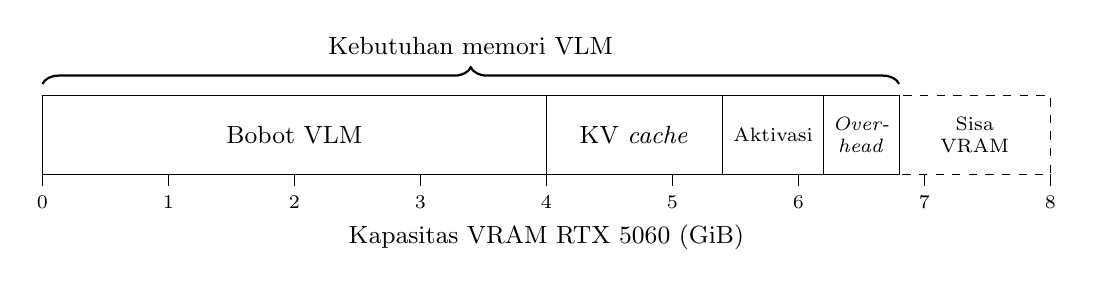
\begin{tikzpicture}[x=1.6cm, y=1cm]
        \draw (0,0) rectangle (4,1) node[midway, align=center, font=\small] {Bobot VLM};
        \draw (4,0) rectangle (5.4,1) node[midway, align=center, font=\small] {KV \textit{cache}};
        \draw (5.4,0) rectangle (6.2,1) node[midway, align=center, font=\scriptsize] {Aktivasi};
        \draw (6.2,0) rectangle (6.8,1) node[midway, align=center, font=\scriptsize] {\textit{Over-}\\\textit{head}};
        \draw[dashed] (6.8,0) rectangle (8,1) node[midway, align=center, font=\scriptsize] {Sisa\\VRAM};
        \foreach \x in {0,1,...,8} { \draw (\x,0) -- (\x,-0.15) node[below, font=\scriptsize] {\x}; }
        \node[font=\small] at (4,-0.8) {Kapasitas VRAM RTX 5060 (GiB)};
        \draw[decorate, decoration={brace, amplitude=6pt}, thick] (0,1.15) -- (6.8,1.15) node[midway, above=7pt, font=\small] {Kebutuhan memori VLM};
    \end{tikzpicture}}
    \caption{Ilustrasi Komponen Kebutuhan Memori VLM pada VRAM GPU}
    \label{fig:vram}
\end{figure}

\subsection{\textit{Vision-Language Model} (VLM)}
\textit{Vision-Language Model} (VLM) adalah model multimodal yang memproses masukan berupa citra dan teks secara bersamaan untuk menghasilkan keluaran berupa teks \cite{ref6}. Arsitektur VLM generatif umumnya terdiri atas enkoder visual berbasis \textit{Vision Transformer} (ViT) yang mengubah citra menjadi vektor fitur, proyektor antar-modalitas yang memetakannya ke ruang token teks, dan \textit{Large Language Model} (LLM) sebagai dekoder yang membangkitkan jawaban secara autoregresif token demi token, sebagaimana diilustrasikan pada Gambar \ref{fig:vlm} \cite{ref6}. Salah satu tugas utama VLM adalah \textit{Visual Question Answering} (VQA), yaitu menjawab pertanyaan berbahasa alami mengenai isi suatu citra, yang dapat dikerjakan secara \textit{zero-shot} tanpa pelatihan tambahan pada kelas atau domain tertentu \cite{ref6}. Kemampuan ini memungkinkan VLM menjawab pertanyaan yang tidak dapat ditangani detektor \textit{closed-set}, misalnya apakah seseorang berperan sebagai pegawai atau pelanggan, sehingga seluruh pengujian VLM dalam penelitian ini dirumuskan sebagai kueri VQA pada \textit{frame} tunggal \cite{ref22} dengan \textit{prompt} yang seragam untuk setiap model. Pada video pengawasan, VLM mampu menalar kejadian anomali tanpa pelatihan tambahan, tetapi menuntut sumber daya komputasi yang besar sehingga pada perangkat berkapasitas terbatas memerlukan kompresi \cite{ref14, ref22}.

\begin{figure}[htbp]
    \centering
    \resizebox{\textwidth}{!}{%
    \begin{tikzpicture}[node distance=0.6cm,
        blok/.style={draw, rounded corners, minimum height=1.2cm, text width=2.3cm, align=center, font=\small},
        panah/.style={-{Stealth[length=2.5mm]}, thick}]
        \node[blok] (img) {Citra / \textit{crop} CCTV};
        \node[blok, right=of img] (enc) {Enkoder Visual (ViT)};
        \node[blok, right=of enc] (proj) {Proyektor (MLP / linear)};
        \node[blok, below=0.9cm of img] (txt) {Pertanyaan teks (\textit{prompt} VQA)};
        \node[blok, below=0.9cm of proj] (tok) {\textit{Tokenizer} teks};
        \node[blok, minimum height=3.3cm, right=1.0cm of proj.south east, anchor=north west, yshift=0.6cm] (llm) {LLM\\(dekoder \textit{transformer})};
        \node[blok, right=of llm] (ans) {Jawaban teks (contoh: ``Ya'')};
        \draw[panah] (img) -- (enc);
        \draw[panah] (enc) -- node[above, font=\scriptsize] {fitur} (proj);
        \draw[panah] (txt) -- (tok);
        \draw[panah] (proj.east) -- node[above, font=\scriptsize] {token visual} (proj.east -| llm.west);
        \draw[panah] (tok.east) -- node[below, font=\scriptsize] {token teks} (tok.east -| llm.west);
        \draw[panah] (llm) -- (ans);
    \end{tikzpicture}}
    \caption{Arsitektur Umum \textit{Vision-Language Model} Generatif (Diolah dari \cite{ref6})}
    \label{fig:vlm}
\end{figure}

Keempat VLM yang diuji merupakan variabel bebas pertama, mewakili keluarga model terbuka yang berbeda dalam enkoder visual, LLM, dan ukuran sekitar 2--4 miliar parameter, dengan estimasi memori bobot pada Tabel \ref{tab:model} yang dihitung dari jumlah parameter dan jumlah \textit{byte} per parameter (Subbab \ref{sub:kuantisasi}) sehingga kebutuhan aktual lebih besar setelah ditambah KV \textit{cache}, aktivasi, dan \textit{overhead}. PaliGemma 2 menggabungkan enkoder SigLIP dengan LLM Gemma 2, dan varian \textit{mix} dipakai agar model dapat langsung menjawab kueri VQA tanpa \textit{fine-tuning}\footnote{Spesifikasi resmi model: \url{https://huggingface.co/google/paligemma2-3b-mix-448}}, sedangkan Qwen2.5-VL varian \textit{Instruct} memproses citra pada resolusi aslinya secara dinamis sehingga jumlah token visual dan KV \textit{cache} bergantung pada ukuran masukan\footnote{Spesifikasi resmi model: \url{https://huggingface.co/Qwen/Qwen2.5-VL-3B-Instruct}}. InternVL2.5 4B menggabungkan enkoder InternViT-300M dengan LLM Qwen2.5-3B melalui proyektor \textit{Multi-Layer Perceptron} (MLP) \cite{ref29}, sedangkan Moondream2 adalah VLM ringkas berukuran sekitar 1,9 miliar parameter yang menggabungkan SigLIP dengan Phi-1.5\footnote{Spesifikasi resmi model: \url{https://huggingface.co/vikhyatk/moondream2}} \cite{ref14} dan telah dipakai untuk mendeskripsikan insiden jalan raya \cite{ref31}. Pengukuran awal pada RTX 5060 mencatat bobot BF16 InternVL2.5 4B sebesar 7,02 GiB (sekitar 7,5 GB) dan bobot BF16 Qwen2.5-VL-3B diperkirakan sekitar 7,5 GB, sehingga keduanya hampir menghabiskan VRAM yang dapat dipakai aplikasi dan paling bergantung pada kuantisasi, sedangkan Moondream2 (sekitar 3,8 GB pada BF16) diperkirakan dapat berjalan tanpa kuantisasi. Perbedaan ukuran dan rancangan keempat model diperkirakan memengaruhi jejak memori, latensi, dan tingkat halusinasi, dengan Moondream2 sebagai model terkecil yang menjadi batas bawah untuk menguji apakah pengurangan parameter berdampak lebih besar terhadap halusinasi dibanding kuantisasi.

\begin{table}[htbp]
    \centering
    \caption{Spesifikasi dan Estimasi Memori Bobot VLM yang Diuji}
    \label{tab:model}
    \renewcommand{\arraystretch}{1.3}
    \small
    \begin{tabular}{|p{2.6cm}|p{2.4cm}|p{2.2cm}|c|c|c|c|}
    \hline
    \multirow{2}{*}{\textbf{Model}} & \multirow{2}{*}{\textbf{Enkoder Visual}} & \multirow{2}{*}{\textbf{LLM}} & \multirow{2}{*}{\textbf{Param.}} & \multicolumn{3}{c|}{\textbf{Estimasi Memori Bobot (GB)}} \\
    \cline{5-7}
    & & & & \textbf{BF16} & \textbf{INT8} & \textbf{NF4} \\
    \hline
    PaliGemma 2 3B & SigLIP-So400m & Gemma 2 2B & $\pm$3,0B & 6,0 & 3,0 & 1,5 \\
    \hline
    Qwen2.5-VL-3B & ViT \textit{window attention} & Qwen2.5 3B & $\pm$3,8B & 7,5 & 3,8 & 1,9 \\
    \hline
    InternVL2.5 4B \cite{ref29} & InternViT-300M & Qwen2.5 3B & $\pm$3,7B & 7,4 & 3,7 & 1,9 \\
    \hline
    Moondream2 & SigLIP & Phi-1.5 & $\pm$1,9B & 3,8 & 1,9 & 1,0 \\
    \hline
    \end{tabular}

    % REVISI R7: catatan estimasi ditambahkan (enkoder visual dan proyektor tetap BF16)
    \vspace{1ex}
    {\footnotesize Catatan: estimasi INT8 dan NF4 mengasumsikan seluruh parameter dikuantisasi. Karena enkoder visual dan proyektor dipertahankan pada BF16 (Subbab \ref{sec:persiapan}), kebutuhan aktualnya lebih besar, terutama pada NF4.\par}
\end{table}

\subsection{Presisi dan Kuantisasi Bobot: BF16, INT8, dan NF4}
\label{sub:kuantisasi}
Presisi bobot menyatakan jumlah bit dan format bilangan yang digunakan untuk menyimpan setiap bobot model, sehingga menentukan besar memori yang ditempati dan seberapa halus nilai bobot direpresentasikan. Penelitian ini menguji tiga tingkat presisi sebagai variabel bebas kedua. BF16 (\textit{Brain Floating Point} 16-bit) adalah format bilangan titik mengambang 16-bit dengan 1 bit tanda, 8 bit eksponen, dan 7 bit mantisa, yang umum digunakan dalam pelatihan jaringan saraf dalam dan di sini dipakai sebagai presisi asli tanpa kuantisasi. INT8 adalah representasi bobot sebagai bilangan bulat 8-bit. \textit{NormalFloat} 4-bit (NF4) adalah tipe data 4-bit yang dirancang optimal secara teori informasi untuk bobot yang berdistribusi normal, dengan 16 nilai kuantil distribusi normal baku sebagai nilai representasinya \cite{ref35}. Dampak langsung presisi terhadap memori dapat diestimasi dari jumlah parameter dikalikan jumlah \textit{byte} per parameter, yaitu 2 \textit{byte} untuk BF16, 1 \textit{byte} untuk INT8, dan sekitar 0,5 \textit{byte} untuk NF4. Estimasi ini belum memperhitungkan faktor skala, konstanta normalisasi, dan lapisan yang tetap disimpan dalam presisi tinggi, sehingga nilai aktual sedikit lebih besar.

Kuantisasi adalah proses menurunkan presisi bobot, yaitu merepresentasikan bobot berpresisi tinggi menggunakan tipe data berpresisi rendah sehingga kebutuhan memori berkurang. Teknik ini dibutuhkan pada perangkat berkapasitas terbatas, yang memiliki keterbatasan dalam daya pemrosesan, memori, dan energi sehingga memerlukan kompresi model seperti kuantisasi, pemangkasan, dan distilasi \cite{ref14}. Kuantisasi pasca-pelatihan (\textit{post-training quantization}) dilakukan setelah model selesai dilatih sehingga tidak memerlukan pelatihan ulang. Pada prinsipnya, setiap bobot dipetakan ke salah satu dari sejumlah nilai diskret yang terbatas menggunakan faktor skala, dan selisih antara bobot asli dan bobot hasil dekuantisasi disebut galat kuantisasi, yang menjadi sumber penurunan akurasi model. Presisi INT8 dihasilkan oleh metode seperti LLM.int8(), yang memakai faktor skala per vektor dan menangani sebagian kecil dimensi fitur berskala besar (\textit{outlier}) secara terpisah dalam presisi 16-bit, serta dilaporkan mengurangi memori inferensi sekitar setengahnya tanpa penurunan kinerja pada model berukuran besar \cite{ref34}. Presisi NF4 dihasilkan oleh metode QLoRA, yang membagi bobot ke dalam blok, menormalisasi setiap blok dengan nilai mutlak maksimumnya ke rentang $-1$ sampai $1$, lalu memetakan setiap nilai ke nilai NF4 terdekat, sedangkan konstanta normalisasi setiap blok dikuantisasi sekali lagi (\textit{double quantization}) untuk menekan memori tambahan \cite{ref35}. Penghematan memori belum tentu mempercepat inferensi, dan penurunan presisi berpotensi melemahkan kemampuan model dalam memverifikasi isi citra sehingga meningkatkan kecenderungan halusinasi. Hubungan antara penghematan memori, latensi, dan perubahan halusinasi inilah yang diukur dalam penelitian ini.

\subsection{Halusinasi Objek dan Evaluasi POPE}
Halusinasi objek adalah kondisi ketika VLM menyatakan keberadaan objek yang tidak terdapat pada citra, dan paling sering terjadi pada objek yang sering muncul dalam data latih atau sering hadir bersama objek lain \cite{ref9}. Pada CCTV, halusinasi berarti alarm palsu, misalnya menyatakan adanya aktivitas transaksi yang tidak pernah terjadi, sehingga tingkat halusinasi menjadi variabel terikat yang krusial dalam menilai kelayakan VLM, terlebih karena penurunan presisi akibat kuantisasi berpotensi meningkatkannya. \textit{Polling-based Object Probing Evaluation} (POPE) menilai halusinasi melalui kueri biner berbentuk ``Apakah terdapat \textless objek\textgreater{} pada citra?'', dengan kueri positif dari objek yang ada pada anotasi dan kueri negatif dari objek yang tidak ada, yang dipilih secara acak (\textit{random}), paling sering muncul (\textit{popular}), atau sering muncul bersamaan dengan objek pada citra (\textit{adversarial}) \cite{ref9}. Format biner ini membuat evaluasi lebih stabil dibanding metode berbasis \textit{caption} yang dipengaruhi gaya keluaran model, dan jawaban model dikelompokkan ke dalam matriks konfusi seperti pada Gambar \ref{fig:konfusi} \cite{ref9}.

\begin{figure}[htbp]
    \centering
    \begin{tikzpicture}[sel/.style={draw, minimum width=4.2cm, minimum height=1.8cm, text width=3.8cm, align=center, font=\small}]
        \node[sel] (tp) at (0,0) {\textbf{TP}\\Objek ada,\\dijawab ``Ya''};
        \node[sel] (fn) at (4.2,0) {\textbf{FN}\\Objek ada,\\dijawab ``Tidak''};
        \node[sel] (fp) at (0,-1.8) {\textbf{FP (halusinasi)}\\Objek tidak ada,\\dijawab ``Ya''};
        \node[sel] (tn) at (4.2,-1.8) {\textbf{TN}\\Objek tidak ada,\\dijawab ``Tidak''};
        \node[font=\small\bfseries, above=2pt of tp] {Prediksi ``Ya''};
        \node[font=\small\bfseries, above=2pt of fn] {Prediksi ``Tidak''};
        \node[font=\small\bfseries, left=4pt of tp, align=right] {Objek\\ada};
        \node[font=\small\bfseries, left=4pt of fp, align=right] {Objek\\tidak ada};
    \end{tikzpicture}
    \caption{Matriks Konfusi pada Evaluasi Halusinasi Berbasis POPE (Diolah dari \cite{ref9})}
    \label{fig:konfusi}
\end{figure}

Berdasarkan matriks konfusi tersebut, POPE melaporkan metrik \textit{accuracy}, \textit{precision}, \textit{recall}, F1-\textit{score}, dan rasio jawaban ``Ya'' \cite{ref9}, sedangkan penelitian ini mendefinisikan \textit{Object Hallucination Rate} (OHR) sebagai proporsi kueri negatif yang dijawab ``Ya'' oleh model, sebagaimana dirumuskan pada Persamaan \eqref{eq:ohr}. Nilai OHR yang tinggi menandakan model mudah berhalusinasi, sedangkan rasio jawaban ``Ya'' jauh di atas 50\% menunjukkan kecenderungan selalu mengiyakan. Perubahan OHR akibat kuantisasi dihitung sebagai selisih antara OHR model terkuantisasi dan OHR model berpresisi asli (BF16), sebagaimana Persamaan \eqref{eq:dohr}.
\begin{equation}
OHR = \frac{FP}{FP + TN} \times 100\%
\label{eq:ohr}
\end{equation}
\begin{equation}
\Delta OHR = OHR_{kuantisasi} - OHR_{asli}
\label{eq:dohr}
\end{equation}
dengan $FP$ jumlah kueri negatif yang dijawab ``Ya'' dan $TN$ yang dijawab ``Tidak''.

\subsection{Metrik Evaluasi Klasifikasi dan Kinerja Inferensi}
Akurasi klasifikasi peran dan jawaban POPE dievaluasi menggunakan matriks konfusi, dengan kelas positif berupa pegawai atau objek ada, melalui \textit{accuracy}, \textit{precision}, \textit{recall}, dan F1-\textit{score} sebagaimana Persamaan \eqref{eq:acc} hingga \eqref{eq:f1} \cite{ref2}.
\begin{equation}
Accuracy = \frac{TP + TN}{TP + TN + FP + FN}
\label{eq:acc}
\end{equation}
\begin{equation}
Precision = \frac{TP}{TP + FP}, \qquad Recall = \frac{TP}{TP + FN}
\label{eq:pr}
\end{equation}
\begin{equation}
F1 = 2 \times \frac{Precision \times Recall}{Precision + Recall}
\label{eq:f1}
\end{equation}
Kinerja inferensi dinilai dari penggunaan memori GPU, status OOM, dan latensi, yaitu waktu sejak kueri dan citra diterima hingga jawaban selesai dibangkitkan. Pembangkitan teks autoregresif menyumbang lebih dari 85\% latensi ujung ke ujung \cite{ref24}. Latensi dilaporkan sebagai rata-rata dari sejumlah pengulangan kueri sebagaimana Persamaan \eqref{eq:lat}.
\begin{equation}
\bar{t} = \frac{1}{N} \sum_{i=1}^{N} \left(t_{selesai,i} - t_{mulai,i}\right)
\label{eq:lat}
\end{equation}
dengan $N$ jumlah kueri serta $t_{mulai,i}$ dan $t_{selesai,i}$ waktu mulai dan selesai kueri ke-$i$.
